
This section is organied as follows. First, the motion and static vector generation procedure is discussed. Then,
our proposed method for fusioning of these two vectors, is explained. Afterwards, the process of exploiting temporal dynamics of 
sub events, is discussed. 


\subsection{Motion Features}
\subsubsection{Low level motion descriptor}
First, it is needed to have a pixel level descriptor to identify moving points in the video. Dense trajectories is a powerful
pixel level algorithm, which captures the motion, and track it across several frames. Therefore, in this work, 
dense trajectories is chosen as the low level descriptor, for capturing raw motion.

\subsubsection{Clustering}

Initially, dense trajectories are created for every frame in the video.
Then, in order to isolate each sub area in a frame, which contains significant movement, DBScan clustering is applied on the 
calculated trajectory points.
Our clustering algorithm is illustrated in the pseudo code Algorithm~\ref{alg:Clustering algorithm}. Empirically, we use 8 and 10 as epsilon and minpoint parameters.



\begin{algorithm}
 \caption{}
   \label{alg:Clustering algorithm}
    \begin{algorithmic}[1]
      \Function{dbScan}{$Dataset, epsilon, MinPoints$}
        \State $Cluster = 0$
        \For{$each$ $P$ in $Dataset$}
	  \If{$P$ is $visited$}
	    \State{$continue$}
	  \EndIf
            \State mark $P$ as $visited$
            \State $NeighborPts = getAllPoints(P, epsilon)$
          \If{$size(NeighborPts) < MinPoints$}
          \State{mark $P$ as $NOISE$}
          \Else
          \State{$Cluster$ = next cluster}
          \State{$addToCluster(P, NeighborPts, Cluster, epsilon, MinPoints)$}
          \EndIf
        \EndFor
       \EndFunction
       
       \Function{addToCluster}{$P, NeighborPts, Cluster, epsilon, MinPoints$}
	\State $add P to cluster Cluster$
	\For{$each$ $point$ $np$ in $NeighborPts$}
	  \If{$P$ is $not$ $visited$}
	    \State $mark$ $np$ as $visited$
	    \State $NeighborPts' = getAllPoints(np, epsilon)$
	    \If {$size(NeighborPts') >= MinPoints$}
            \State $NeighborPts = NeighborPts joined with NeighborPts'$
            \EndIf
	    
	  \EndIf
	  \If{$np$ is $not$ yet member of any cluster}
         \State $add$ $np$ to cluster $Cluster$
         \EndIf
	\EndFor
       \EndFunction
       
       \Function{getAllPoints}{$P, epsilon$}
       \State $return$ all points within $P$'s $epsilon$-neighborhood (including $P$)
       \EndFunction
\end{algorithmic}

\end{algorithm}


Even though there are many regions, which contain motion, in a video, some are not significant, nor descriptive.
Those moving regions can be neglected without loss of performance. Therefore, after clustering each trajectory point in to cluster groups, 
non-significant cluster groups are neglected.
This is done, in order to prevent the algorithm focusing on small random moving areas in a video, and to only create motion tubes along areas, which are significant and descriptive.
Therefore, all the clusters, which are not at least 50\% in area size, of the largest cluster of the frame, are discarded.

After identifying the initial candidate clusters, for creating action boxes, further processing is done to each cluster to ensure that they 
contain only the important moving areas, according to the Algorithm~\ref{alg:boundary removal}. For each point, the chebychev distance, from the centroid of the cluster, is calculated,
as in
equation \ref{eq:chebichev}, and, furthest 20\% of the points, with respect to the total number of points, are discarded from the cluster. The reason behind the choice of chebychev 
distance, over euclidean distance, is that, a symmetric square shaped cluster groups are obtained, rather than a circle. Which makes it
easier to track moving areas, and create motion tubes. 

\begin{equation}\label{eq:chebichev}
 D_{chebychev} = max(|X_{2} - X_{1}|,|Y_{2}-Y_{1}|)
\end{equation}

\begin{algorithm}
   \caption{}
   \label{alg:boundary removal}
    \begin{algorithmic}[1]
     \Function{formatCluster}{$inCluster, maxChebichevDistance$}
	\State {$maxD_{chebichev}$ = $maxChebichevDistance$}
	\State {$totalPoints$ = $getTotalPoints(inCluster, maxD_{chebichev})$}
	\State $currentPoints$ = $totalPoints$
	\While{$true$}
	  \If{$number_of_count_currentPoints<number_of_count_totalPoints*80/100$}
	    \State return $all the points bellong to currentPoints$
	  \EndIf
	  \State {$maxD_{chebichev}$ = $maxD_{chebichev}$ - 1}
	  \State {$currentPoints$ = $getTotalPoints(inCluster, maxD_{chebichev})$}
	  
	\EndWhile
     \EndFunction

     
\end{algorithmic}
\end{algorithm}

After identifying square shaped interest regions (action boxes), each of them is represented with a vector $b = (x,y,r,f)$, where, $x,y$ are the coordinates
of the top left corner of the box, $r$ is the height/width of the box, and $f$ is the frame number. 


\subsubsection{Motion Tubes}
Since our work models the time evolution of sub activities, within a video, we divide each input video $V_{i}$ into temporal segments $f(V_{i}) = [v_{i,1},
v_{i,2},.....v_{i,n}]$,
and create features for each individual segment separately. Therefore, after creating the action boxes for each video segment,
the action boxes within a segment $v_{i,t}$ can be represented as per equation, 

\begin{equation} 
\label{eqn:action box}
\begin{split}
\MoveEqLeft
 g(v_{i,t}) = \big\{[b_{t,1,1},b_{t,1,2},...,b_{t,1,q}],\\
 & [b_{t,2,1},b_{t,2,2},...,b_{t,2,p}],...,[b_{t,n,1},b_{t,n,2},...,b_{t,n,k}]\big\}
\end{split}
\end{equation}

Where $b_{t,j,k}$ is the $k^{th}$ action box in $j^{th}$ frame of the $t^{th}$ video segment. Note that the number of
action boxes differ from frame to frame.

Therfore, Before linking the action boxes to create motion tubes, further pre processing is needed to ensure same number of action
boxes exists in every frame, within a video segment. Otherwise, different motion tubes could become joined halfway though the video, and the 
effort to capture dynamics of each moving object separately, is disturbed. 

First, the rounded down mean number of action boxes, per a frame,
is calculated. And we iterate through each frame from frame number 1, until we come to a frame, which has that number of action boxes.

Then from that frame, we propagate forward and back along the frames, either to eliminate, or add action boxes.The procedure is explained
below. 

If the action box count in a particular frame, is larger than the previous frame, the smallest excess number of action boxes are removed.
In the case, where action box count is lower than the previous frame, linear regression for each value $x,y$ and $r$ of vector $b = (x,y,r,f)$,
up to that frame, is used to create artificial action boxes, until the number of action boxes match the mean number of action boxes, as in
equation \ref{eqn:linear regression}.
\begin{equation}
\label{eqn:linear regression}
\begin{bmatrix}
    Y_{1}     \\
    Y_{2}     \\
    \hdotsfor{1} \\
    Y_{n}     
\end{bmatrix}
=
\begin{bmatrix}
    1 & X_{1}     \\
    1 & X_{2}     \\
    \hdotsfor{2} \\
    1 & X_{n}     
\end{bmatrix}
*
\begin{bmatrix}
    \beta_{0}     \\
    \beta_{1}      
\end{bmatrix}
+
\begin{bmatrix}
    \epsilon_{1}     \\
    \epsilon_{2}    \\
    \hdotsfor{1} \\
    \epsilon_{n}    
\end{bmatrix}
\end{equation}

Where, $Y, X$ would be either $x,y$ or $r$. Then least square method is used to minimize the error matrix $\sum{\epsilon^2}$, and find the 
values for $\beta_{1}$ and $\beta_{0}$. Afterwards, using these values, missing action boxes are predicted.
Note that $n$ increases as the observed action boxes
increases, hence the prediction becomes more accurate. Note, after this processing, equation \ref{eqn:action box}
is transformed in to equation \ref{eqn:action box transformed}, 
which illustrates that the number of action boxes per frame is equal for all the frames, within a video segment. 

\begin{equation}
\label{eqn:action box transformed}
\begin{split}
\MoveEqLeft
 h(g(v_{i,t})) = \big\{[b_{t,1,1},b_{i,1,2},...,b_{t,1,k}],\\
 & [b_{t,2,1},b_{t,2,2},...,b_{t,2,k}],...,[b_{t,n,1},b_{t,n,2},...,b_{t,n,k}]\big\}
\end{split}
\end{equation}


The following procedure
is used to link the action boxes in consecutive frames.

Assume $b_{t,k,1}$,$b_{t,k,2}$,...,$b_{t,k,n}$ and $b_{t,k+1,1}$,$b_{t,k+1,2}$,...,$b_{t,k+1,n}$  are action boxes in two 
consecutive frames at time $k,k+1$. Then, following distance matrix is calculated.


 
\begin{equation}
D=\begin{bmatrix}
    D_{11}       & D_{12} & D_{13} & \dots & D_{1k} \\
    D_{21}       & D_{22} & D_{23} & \dots & D_{2k} \\
    \hdotsfor{5} \\
    D_{k1}       & D_{k2} & D_{k3} & \dots & D_{kk}
\end{bmatrix}
\end{equation}


Where, $D_{i,j}$ is the euclidean distance, between the centroids of $i^{th}$ action box in $k^{th}$ frame and $j^{th}$ action box in $(k+1)^{th}$ frame. 
Then, $u^{th}$ action box at $k+1$, and $1^{st}$ action box at $k$ is linked, where $u$ is calculated using,


\begin{equation}
u=\underset{j\in J}{argmin_j}\{D_{1,j}\}, J=\{1,2,...,l\}
\end{equation}

Then, the $1^{st}$ row and the $u^{th}$ column is removed from the distance matrix, and the same process is applied repeatedly
to link each of the action boxes at $k$ with $k+1$. By this removal process, we avoid combining of motion tubes in half-way through 
the video segment, and keep them isolated from each other, which is vital to capture the dynamics separately, for each moving object.




Finally, we create matrix $M_{i}$ which encodes all the information of motion tubes, in a particular video segment.
\begin{equation}
M=\begin{bmatrix}
    1       & 1 & x_{1,1} & y_{1,1} & r_{1,1} \\
    1       & 2 & x_{1,2} & y_{1,2} & r_{1,2} \\
    \hdotsfor{5} \\
    1       & n & x_{1,n} & y_{1,n} & r_{1,n} \\
    2       & 1 & x_{2,1} & y_{2,1} & r_{2,1} \\
    2       & 2 & x_{2,2} & y_{2,2} & r_{2,2} \\
    \hdotsfor{5} \\
    2       & n & x_{2,n} & y_{2,n} & r_{2,n} \\
    \hdotsfor{5} \\
    z       & 1 & x_{z,1} & y_{z,1} & r_{z,1} \\
    z       & 2 & x_{z,2} & y_{z,2} & r_{z,2} \\
    \hdotsfor{5} \\
    z       & n & x_{z,n} & y_{z,n} & r_{z,n} \\
    
\end{bmatrix}
\end{equation}

Where, columns represent, the frame number, action box number, $x$ coordinate of the top left corner,
$y$ coordinate of the top left corner, and the width/height of the action box, respectively. 

\subsubsection{Histogram Oriented Optic Flows(HOOF)}
Since each action box, in a particular motion tube, may differ in size, we take $R = max(r_{i})$, for $\forall{i}$
where $r_{i}$ is the $i^th$ action box of the motion tube. Then we redraw the action boxes around thier centroids, having width/length as $R$.
After identifying the $k$ number of motion tubes (k is a variable) for each video segment $v_{i,n}$, the optic flows along each motion tube,
, are calculated, using Lucas \textit{et. al}.
After that, Histogram-Oriented-Optic-Flows, for each motion tube is created. We create HOOFs for every
action box within a motion tube. Each optic flow vector within a spatio-temporal action box within a motion tube, is binned according
to its primary angle from the horizontal axis and weighted according to its magnitude.  Therefore, all optical flow vectors, $z=[x,y]^T$ with direction,
$\theta = tan^{-1}(\frac{x}{y})$ in the range,

\begin{equation}
- \frac{\pi}{2} + \pi\frac{b-1}{B} \leq \theta < -\frac{\pi}{2} + \pi\frac{b}{B}
\end{equation}

will contribute by a weight of $\sqrt{x^2 + y^2}$ to the sum in bin $b$, $1 \leq b \leq B$ out of a total of
$B$ bins. Finally, the histogram is normalized. We choose 100 as the bin number.

\subsubsection{Bag of HOOFs}
We use a bag of features method to create a motion descriptor for each video segment. First, we create a code book for HOOF vectors. 
100000 vectors are randomly selected, from all the HOOF vectors, of all the video segments, in all video classes. 
Then these 100000 vectors are clustered using k-means clustering, and 1000 cluster heads
are identified. We choose the number of cluster heads as 1000, because, the dimensions of final motion descriptors are needed to be same as
static descriptors, which is explained later. Then for each video segment $v_{i,n}$, a histogram is calculated as following. 

for each, 
\begin{equation}
k \in \big\{1,2,......l\big\}
\end{equation}

we calculate,
\begin{equation}
p = \underset{j\in J}{argmin_{j}}(T_{j}-h_{n,k}), J=\{1,2,...,1000\}
\end{equation}

Where, $h_{n,k}$ is the $k^{th}$ HOOF vector of the $n^{th}$ video segment, and $T_{j}$ is the $j^{th}$ cluster head. And then,
histogram values are incremented as in,

\begin{equation}
H_{n}(p) = H_{n}(p)+1
\end{equation}

where $H_{n}(p)$ is the $p^{th}$ value, $1<p<1000$, of histogram of $n^{th}$ video segment $v_{i,n}$. After calculating the histogram vector $H_{n}$, for every video segment $v_{i,n}$, 
this $H = [H_{1},H_{2},.......H_{n}]$ is the vector time series, which encodes the time evolution of motion information, in the video.

\begin{figure}
  \centering
  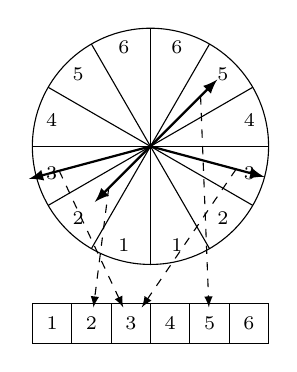
\begin{tikzpicture}[x=1cm, y=1cm, every node/.append style={text=black, font=\scriptsize}]
\def\r{1.5}
	\draw (0,0) coordinate (o) circle (\r);
	\foreach \theta in {-90, -60, ..., 240}
	{
		\draw (o) -- (\theta:\r);
	}
	\foreach \theta/\l in {-60/1, -30/2, 0/3, 30/4, 60/5, 90/6}
	{
		\node at  (\theta - 15:1.3) {$\l$};
	}	
	\foreach \theta/\l in {-90/1, -120/2, -150/3, -180/4, -210/5, -240/6}
	{
		\node at  (\theta - 15:1.3) {$\l$};
	}		
	
	\foreach \theta/\r/\t in {-15/1.5/1, 45/1.2/2, -135/1/3, -165/1.6/4}
	{
		\draw[-latex, thick] (o) -- (\theta:\r ) coordinate [near end] (t\t);
	}
	
	\foreach \i/\l in {-1.25/1, -0.75/2, -0.25/3, 0.25/4, 0.75/5, 1.25/6 }
	{
		\draw (\i-0.25, -2) rectangle ++(0.5, -0.5);
		\node (a\l) at (\i, -2.25) {$\l$} ;
	}
	
	\draw[-latex, dashed] (t1) -- (a3);
	\draw[-latex, dashed]  (t2) -- (a5);
	\draw[-latex, dashed]  (t3) -- (a2);
	\draw[-latex, dashed]  (t4) -- (a3);
	
	
\end{tikzpicture} 
  \caption{Test Figure}\label{fi:hoof}
\end{figure}


\subsection{Static Features}

In order to create static descriptors, we create a CNN of 1000 output classes, and train it on image-net dataset. The architecture is shown in figure \ref{fi:cnn}.
After 30 epochs, the training is stopped and used on each individual frame of each video segment. Then, the output vectors of the CNN,
are averaged 
along indexes, and a static descriptor $s_{i}$ is obtained foe each video segment $v_{i}$. Following the 
procedure for every $v_{i}$, finally, we have a vector time series 
$S =[s_{1}, s_{2},...s_{n}]$, representing the static time evolution of the whole video. 

\begin{figure*}
  \centering
  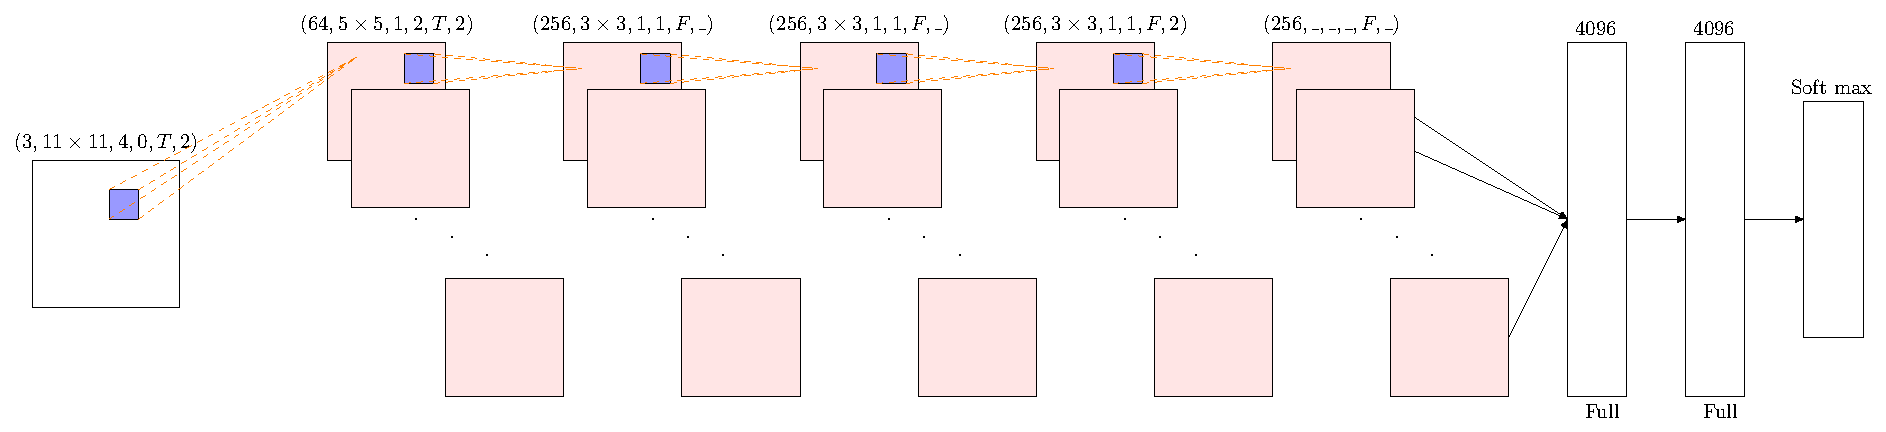
\includegraphics[scale=0.5]{./figures/nw.pdf} 
  \caption{Overall methodology}\label{fi:cnn}
\end{figure*}

\subsection{Fusioning of static and motion features}
This work strongly relies on the philosophy, that both static and motion information
are vital for action recognition. Therefore, the following mathematical models is used
to fuse the static and motion vectors. We do our mathematical derivation based on the Cholesky transformation. An 
abstract version of Cholesky transformation is described next. 

Let $P$ and $Q$ be two random variables of unknown correlation. These random variables can be
transformed into two new random variables ($R$ and $S$) with a known correlation of $\rho$, where the 
value of $\rho$ can be chosen at will. The transformation can be performed as follows.

\[
\begin{bmatrix}
    R     \\
    S     
\end{bmatrix}
=
\begin{bmatrix}
    1  & 0 \\
    \rho  & \sqrt{1-\rho^2}    
\end{bmatrix}
*
\begin{bmatrix}
    P     \\
    Q     
\end{bmatrix}
\]

Therefore,

\begin{equation}
R = P
\end{equation}

\begin{equation}
S = \rho P + \sqrt{1-\rho^2}Q
\end{equation}

The Cholesky transformation guarantees that the correlation between the two random variables
$R$ and $S$ is $\rho$.

Based on the above properties of the Cholesky transformation, we propose the following methodology to fuse the static and
motion vectors.

Let $X$ and $Y$ be static and motion vectors, respectively. Cholesky transformation can be applied to the two vectors $X$ and $Y$, 
with the correlation value $\rho_{1}$.

\[
\begin{bmatrix}
    R     \\
    S     
\end{bmatrix}
=
\begin{bmatrix}
    1  & 0 \\
    \rho_{1}  & \sqrt{1-\rho_{1}^2}    
\end{bmatrix}
*
\begin{bmatrix}
    X    \\
    Y     
\end{bmatrix}
\]

\begin{equation}
R = X
\end{equation}

\begin{equation}
S = \rho_{1} Y + \sqrt{1-\rho_{1}^2}Y
\end{equation}

Similarly, the transformation can be applied to $Y$ and $X$, with the correlation value $\rho_{2}$.


\[
\begin{bmatrix}
    A     \\
    B     
\end{bmatrix}
=
\begin{bmatrix}
    1  & 0 \\
    \rho_{2}  & \sqrt{1-\rho_{2}^2}    
\end{bmatrix}
*
\begin{bmatrix}
    Y    \\
    X     
\end{bmatrix}
\]

\begin{equation}
A = Y
\end{equation}

\begin{equation}
B = \rho_{2} X + \sqrt{1-\rho_{2}^2}X
\end{equation}

Again, the Cholesky transformation guarantees the follwing two properties.


\begin{enumerate}
  \item The correlation between $X$ and $S$ is $\rho_{1}$.
  \item The correlation between $Y$ and $B$ is $\rho_{2}$.
\end{enumerate}

Therefore, if the values of $\rho_{1}$ and $\rho_{2}$ are chosen in such a way that they obey the following
rule,

\begin{equation}
\rho_{2} = \sqrt{1-\rho_{1}^2}
\end{equation}

It can be guaranteed that $S = B$, $\forall X,Y,\rho_{1},\rho_{2}$. Hence, the resultant vector $Z$ can be obtained
by,

\begin{equation}
Z=S=B
\end{equation}

Where the correlation between $Z$ and $X$ is $\rho_{1}$ and the correlation between $Z$ and $Y$ is $\rho_{1}$. This derivation 
leads us to an important intuition. Here $X$ and $Y$ represent the static and the
motion vectors whereas $Z$ represents the resultant vector. By choosing the value of $\rho_{1}$, we can
choose the degree, in which the static features and the motion features contribute,
in deriving the resultant vector. In section 4, it is shown, how this property is used to explore, the optimal contribution of 
static and motion domain information, for recognizing actions. 

\subsection{Capturing temporal evolution}
In our work, a video is represented as $n$
fixed-length segments (n differ for videos of different lengths),  with overlapping frames.  Each segment
is represented with a fusioned vector $c_{t}$. Therefore, each video can be represented as a vector time series 
$C = [c_{t_0},c_{t_1},...c_{t_{n-1}}]$. 

Now, each vector time series could be  analyzed using traditional time series modeling techniques,
such as Auto Regressive Moving Average [1] etc. Where it is possible to obtain features or model parameters to describe the
vector time series. 
But the main drawback of these methods is, they model current values of a series as a function of past values,
and have finite dynamic response to time series input. Also they lack the ability to grasp the internal state 
representations of a complex time series. Recurrent neural nets, on the other hand, maintain hidden layers with directed feedback connections, and hence,
have an infinite dynamic response. While training, it learns internal states of a sequence,
and are usually performed better in modeling complex dynamic temporal patterns of long sequences.


But, it is not ideal to train standard RNNs to solve problems,
which require, learning of long-term temporal dependencies. This is because of the vanishing-gradient problem, which occurs
due to the exponential decay of gradient loss of the function, with respect to time. 

In practice, LSTM(Long short term memory) networks, typically perform better in such cases.
LSTM networks are a special type of RNN, which include a 'memory cell', and as the name suggests,
it can maintain a certain state, in memory, for longer periods of time. 
Also, it has a set of control gates, which is a structured way of controlling removal or addition information to the cell state.
This special architecture gives them the ability to capture longer-term dependencies. In the next section, the operation of a LSTM
network is revisited.

The most important structure of a LSTM unit is its memory cell $C_{t}$, which preserves the state. Basic structure of a LSTM
unit is shown in figure. The memory cell is self connected, and it has three gates(multiplicative units), i.e. input gate, forget gate and 
output gate, which are used to control, how much to store, remove or output long range contextual information of a temporal sequence.

The detailed activation process of the memory cell and three gates are
illustrated as follows:

\begin{equation}
i^{t} = \sigma (W_{xi}x^t + W_{hi}h^{t-1} + W_{ci}c^{t-1} + b_{i})
\end{equation}
\begin{equation}
f^{t} = \sigma (W_{xf}x^t + W_{hf}h^{t-1} + W_{cf}c^{t-1} + b_{f})
\end{equation}
\begin{equation}
c^{t} = f^tc^{t-1} + i^ttanh(W_{xc}x^t + W_{hc}h^{t-1} + b_{c})
\end{equation}
\begin{equation}
o^{t} = \sigma (W_{xo}x^t + W_{ho}h^{t-1} + W_{co}c^{t-1} + b_{o})
\end{equation}
\begin{equation}
h^t = o^ttanh(c^t)
\end{equation}

Where $W$ is the connection weight between two units and $\sigma(.)$ is the sigmoid function.

Since the LSTM network is used only for capturing the temporal dynamic patterns between sub actions, one LSTM layer is enough.
Our LSTM network is shown in figure. As it is seen, the network consists of an input layer, a 128 unit LSTM layer with 0.8 dropout, and
a fully connected softmax output layer. As we have a sequence of activites per one classification, we use many to one approach,
for feeding the fusioned vectors to the network, as shown in figure \ref{fi:lstm}

\begin{figure}
  \centering
  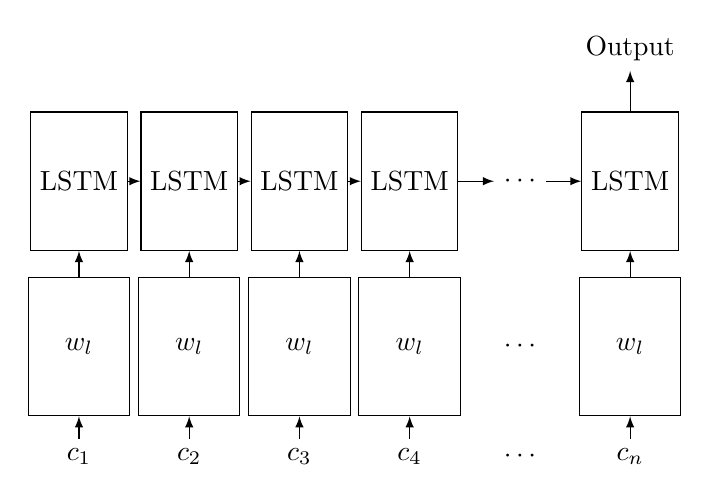
\begin{tikzpicture}[x=0.7cm, y=0.7cm] 
	\foreach \i/\l in {1/1, 2/2, 3/3, 4/4, 6/n}
	{
		\node[draw=black, minimum height=50] (1\i) at (2*\i, 0) {LSTM};
		\node[draw=black, minimum height=50, text width=30, align=center] (2\i) at (2*\i, -3) {$w_l$};
		\node[text width=30, align=center] (3\i) at (2*\i, -5) {$c_\l$};		
	}
	
	\node (15) at (2*5,0) {$\cdots$};
	\node (25) at (2*5,-3) {$\cdots$};
	\node (35) at (2*5,-5) {$\cdots$};	
	
	\foreach  \i/\j in {1/2, 2/3, 3/4, 4/5, 5/6}
	{
		\draw [-latex] (1\i) -- (1\j);
	}
	
	\foreach  \i in {1,2,3,4,6}
	{
		\draw [-latex] (2\i) -- (1\i);
		\draw [-latex] (3\i) -- (2\i);
	}	
	
	\draw[-latex] (16) -- +(0,2) node [anchor=south] {Output};
	

\end{tikzpicture}
  \caption{Test Figure}\label{fi:lstm}
\end{figure}




